\section{Introduction}


\begin{figure*}[t]
    \centering
A    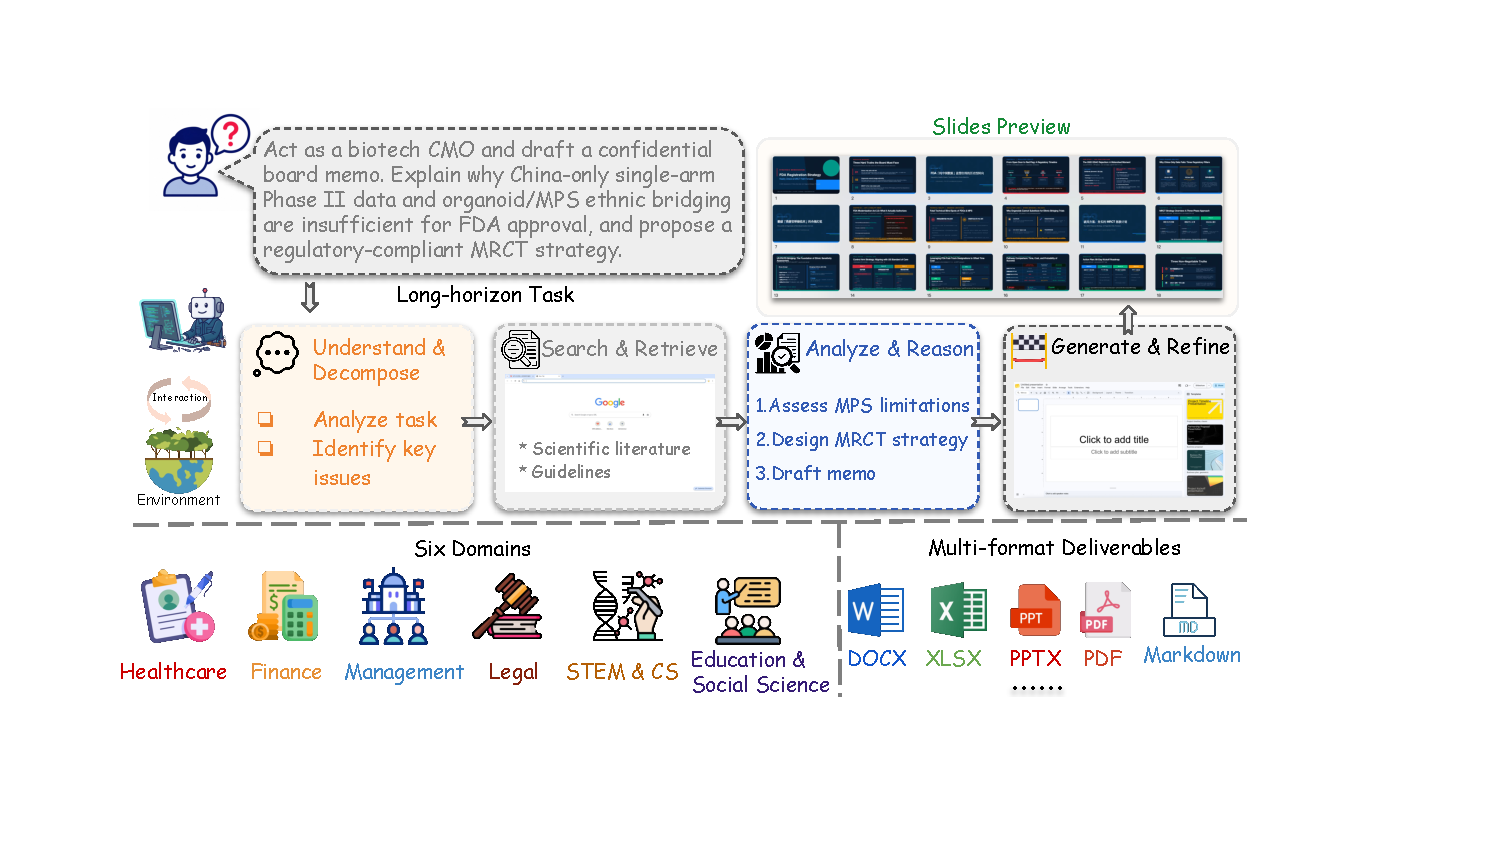
\includegraphics[width=0.9\textwidth]{figures/MainFig.pdf}
    \caption{
    Overview of StartupBench: real AI-product workflows, long-horizon agent execution, six-domain coverage, and multi-format deliverable generation.
    }
    \label{fig:bench_overview}
% \vspace{-6pt}
\end{figure*}

Large language models (LLMs) are increasingly evolving from systems that primarily retrieve information or answer questions\cite{du2026supergpqa,mialon2024gaia,wang2024mmlu} into agents capable of completing complex real-world tasks. Current AI systems are expected to execute end-to-end (E2E) workflows, coordinate multiple capabilities, and produce deliverables that satisfy practical requirements under realistic constraints. As AI becomes increasingly integrated into professional work, autonomously completing user-delegated tasks has become an important measure of model capability. Evaluating whether AI systems can reliably translate their capabilities into professionally usable deliverables is therefore a central challenge for the next generation of benchmarks.



Recent benchmarks have made important progress toward evaluating E2E task execution under realistic settings. Nevertheless, several important limitations remain. First, many benchmark tasks are still largely defined from researchers' perspectives rather than grounded in workflows that have demonstrated practical demand through real-world AI adoption~\cite{phan2025humanity,patwardhan2025gdpval,mialon2024gaia}, limiting their ability to reflect authentic user needs and deliverable requirements. Second, although several benchmarks evaluate complete deliverables~\cite{tang2026workspace,sun2026agents}, their evaluation protocols are often substantially coarser than the deliverables themselves. Real-world work products typically involve numerous functional, structural, formatting, and domain-specific requirements that holistic evaluations cannot faithfully assess. Consequently, existing benchmarks still provide only limited evidence of \textit{how well current models and agents can satisfy complex real-world user requirements and reliably produce professionally usable deliverables}.


To address these limitations, we observe that AI-native startups offer a natural source of real-world AI workflows: their products have been validated through real-world adoption and commercial demand, providing direct evidence that users value and seek to delegate these tasks to AI. We therefore introduce \textbf{StartupBench}, a survey- and interview-driven benchmark that draws on these workflows to capture realistic E2E user requirements across domains. StartupBench spans 97 tasks across 6 primary domains and is built around the following design principles:


\begin{itemize}
\item \textbf{Adoption-grounded task sourcing.} We systematically survey AI-native startups and their products, complemented by product demonstrations and user interviews, to identify workflows with demonstrated real-world demand. We then construct these workflows into benchmark tasks that preserve their core user objectives and practical requirements.


\item \textbf{E2E deliverables.} Each task requires producing the complete deliverables that users ultimately expect in realistic workflows, rather than intermediate outputs or simplified demonstrations.

\item \textbf{Fine-grained rubric-based evaluation.} Each StartupBench task is evaluated using multiple independent rubrics covering distinct dimensions of the expected deliverable, including functionality, structure, formatting, and domain-specific quality, ensuring a comprehensive and faithful assessment of real-world task completion.

\end{itemize}



We evaluate representative models on StartupBench under  unified agentic harness. Results show that even the strongest model successfully completes only about 30\% of benchmark tasks, indicating that current general-purpose systems remain far from reliably producing professionally usable deliverables. Performance varies substantially across domains, with Finance, STEM \& Computer Science and Education \& Humanities proving particularly challenging. Deeper analysis further attributes these failures primarily to  limitations in complex instruction following and domain-specific expertise, highlighting promising directions for future foundation models and agent systems.



To summarize, our contributions are as follows:

\begin{itemize}
    \item We propose a survey- and interview-driven methodology for constructing agent benchmarks from real AI adoption scenarios.
    \item We construct StartupBench, a benchmark built through AI-native startup research, enterprise-user interviews, user-oriented task abstraction, expert data construction, and multi-stage quality control.
    \item We present a comprehensive empirical study of current foundation models and general-purpose agents on startup-derived workflows, providing a practical evaluation signal for assessing whether AI agents are progressing from answering questions toward reliably completing real work.
\end{itemize}


%\subsection{Hello World}
